\titledquestion{Topological Sort}

Given the following DAG, run topological sort with a queue. Write down the vertex you select and update the in-degree \texttt{ind[i]} of all vertices in each iteration.

\textit{Note: When pushing several vertices into the queue at the same time, push them alphabetically. You are NOT required to show your queue at each step.}

\vspace{1cm}

\begin{figure}[htbp]
    \centering
    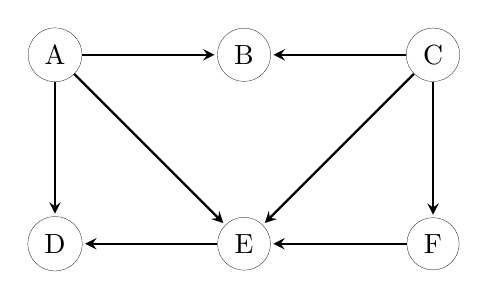
\begin{tikzpicture}[
        > = stealth, % arrow head style
        shorten > = 1pt, % don't touch arrow head to node
        node distance = 1cm, % distance between nodes
        thick, % line style
        scale = 0.8,
    ]
        % Draw the nodes
        \foreach \pos/\i in {
            (-3,3)/A,
            (0,3)/B,
            (3,3)/C,
            (-3,0)/D,
            (0,0)/E,
            (3,0)/F} {
            \node[circle, draw, line width=0.1pt] (\i) at \pos {\i};
        }

        % Draw the edges
        \foreach \b/\e in {
            A/B,
            A/D,
            A/E,
            C/B,
            C/E,
            C/F,
            F/E,
            E/D} {
            \draw[->] (\b) to (\e);
        }
    \end{tikzpicture}\label{fig:Topological_Sort}
\end{figure}
\vspace{0.5cm}

\begin{table}[htbp]
    \begin{center}
        \begin{tabular}{|l|c|l|l|l|l|l|l|}
            \hline
            & vertex & \texttt{ind[A]}    & \texttt{ind[B]}    & \texttt{ind[C]}    & \texttt{ind[D]}    & \texttt{ind[E]} & \texttt{ind[F]}\\ \hline
            initial     & /      & \textcolor{blue}{} & \textcolor{blue}{} & \textcolor{blue}{} & \textcolor{blue}{} & \textcolor{blue}{} & \textcolor{blue}{}   \\ \hline
            iteration 1 &        & \textcolor{blue}{} & \textcolor{blue}{} & \textcolor{blue}{} & \textcolor{blue}{} & \textcolor{blue}{} & \textcolor{blue}{}   \\ \hline
            iteration 2 &        & \textcolor{blue}{} & \textcolor{blue}{} & \textcolor{blue}{} & \textcolor{blue}{} & \textcolor{blue}{} & \textcolor{blue}{}   \\ \hline
            iteration 3 &        & \textcolor{blue}{} & \textcolor{blue}{} & \textcolor{blue}{} & \textcolor{blue}{} & \textcolor{blue}{} & \textcolor{blue}{}   \\ \hline
            iteration 4 &        & \textcolor{blue}{} & \textcolor{blue}{} & \textcolor{blue}{} & \textcolor{blue}{} & \textcolor{blue}{} & \textcolor{blue}{}   \\ \hline
            iteration 5 &        & \textcolor{blue}{} & \textcolor{blue}{} & \textcolor{blue}{} & \textcolor{blue}{} & \textcolor{blue}{} & \textcolor{blue}{}   \\ \hline
            iteration 6 &        & \textcolor{blue}{} & \textcolor{blue}{} & \textcolor{blue}{} & \textcolor{blue}{} & \textcolor{blue}{} & \textcolor{blue}{}   \\ \hline
        \end{tabular}
    \end{center}\label{tab:Topological_Sort_Answer}
\end{table}
\vspace{0.5cm}



\begin{parts}
    \part[3] Fill in the table above.
    \part[2] What is the topological order that you obtain?
    \part[3] How many different topological orders starting with A does this graph have?
    Write them down.
\end{parts}